% Final project for CS 294-73 at Berkeley
% Amirreza Hashemi and Júlio Caineta
% 2017

% Use the standard article template.
\documentclass{article}
\usepackage[utf8]{inputenc}
\usepackage[english]{babel} % English language/hyphenation
\usepackage[super]{nth}
\usepackage[numbers]{natbib}
\usepackage{authblk}
% The geometry package allows for easy page formatting.
\usepackage{geometry}
\geometry{letterpaper}
\usepackage{amssymb}
\usepackage{amsmath}	
% Load up special logo commands.
\usepackage{doc}

% Package for formatting URLs.
\usepackage{url}
\usepackage[hidelinks]{hyperref}

\usepackage{lscape}

%Gantt chart package
\usepackage{xcolor,colortbl}

% A package which allows simple repetition counts, and some useful commands

\usepackage{forloop}
\newcounter{loopcntr}
\newcommand{\rpt}[2][1]{%
  \forloop{loopcntr}{0}{\value{loopcntr}<#1}{#2}%
}
\newcommand{\on}[1][1]{
  \forloop{loopcntr}{0}{\value{loopcntr}<#1}{&\cellcolor{gray}}
}
\newcommand{\onx}[1][1]{
  \forloop{loopcntr}{0}{\value{loopcntr}<#1}{&\cellcolor{orange}}
}
\newcommand{\off}[1][1]{
  \forloop{loopcntr}{0}{\value{loopcntr}<#1}{&}
}

\definecolor{orange}{HTML}{FF7F00}

%%

% Packages and definitions for graphics files.
\usepackage{graphicx}
\usepackage{epstopdf}
\DeclareGraphicsRule{.tif}{png}{.png}{`convert #1 `dirname #1`/`basename #1 .tif`.png}

%\pagestyle{empty}
\date{}
%
% Set the title, author, and date.
%
\title{Implementation of a second order projection method for viscous incompressible flow} 
\author[1]{Amirreza Hashemi}
\author[2]{Júlio Caineta}
\affil[1]{Computational Modeling and Simulation Program, \authorcr
	Department of Mechanical Engineering and Materials Science, University of Pittsburgh}
\affil[2]{Computational Modeling and Simulation Program, \authorcr
	Department of Geology and Environmental Science, University of Pittsburgh}
\affil[ ]{E-mail: \tt {\{amh299, julio.caineta\}@pitt.edu}}
\date{December \nth{15} 2017}

\hypersetup
{
	pdfauthor={Amirreza Hashemi and Júlio Caineta},
	pdfsubject={CS294-73 Project summary},
	pdftitle={CS294-73 Project summary}
}

%
% The document proper.
%
\begin{document}

% Add the title section
\maketitle
\thispagestyle{empty}.

%\pagenumbering{roman}

%
% Body text.
%
\pagebreak
\section*{Summary} 


In the final project, we plan to solve the two dimensional Navier-Stokes equations based on \cite{Bell1991a}. The method is a second-order fractional step scheme, where diffusion-convection equations are firstly solved to determine intermediate velocities, which are then projected onto the space of divergence-free vector fields. The discretization of the projection operator introduced in the original paper will be replaced with an approximate projection derived by Lai \cite{Lai1993a}. Lai's projection method is a modification that accounts for the non-zero divergence of the velocity and has a second order accuracy both in space and time. Finally, convergence and performance of our numerical implementation will be verified by applying the method to vortex spindown in a box, similarly to the test case introduced in the original paper. 

\pagebreak

\section{Introduction and governing equations}

In this project, we aim to reproduce the results of \cite{Bell1991a} and improve it using a projection method that has been developed by Lai \cite{Lai1993a}. The governing equations are the incompressible Navier-Stokes \eqref{eq:nsp} and the continuity in non-dimensional fashion \eqref{eq:cont}.

\begin{equation}
\label{eq:nsp}
\begin{split}
U_t + (U  \cdot \nabla)U = Re \Delta U - \nabla p
\end{split}
 \end{equation}
 \begin{equation}
 \label{eq:cont}
\begin{split}
\nabla \cdot U = 0
\end{split}
 \end{equation}
 In these equations, $U$ is the velocity vector field, $p$ is pressure and $\mathit{Re}$ represents the non-dimensional Reynolds number. For illustration and validation, the physical problem is a vortex spindown in a cavity for two Reynolds numbers (100 and 20000). The length of the box is one in each side, and we consider solid boundary conditions for all the side walls, so that $U_d \cdot n = 0$, where $d$ represents the direction index. The results will consist of a contour plot of vortex spindown and a performance test of the implemented numerical method.


\section{Numerical methods}

The numerical method is a three-step process. The first step is related to an unsplit second-order Godunov method to compute time-centered conservative differences of the nonlinear flux terms $(U \cdot \nabla)U$. The Godunov method is a predictor-corrector method and is used to calculate intermediate velocities. These predicted velocities are then used in a corrector step in which Riemann problems are solved to resolve ambiguities in the upwind direction and the resultant states are used to evaluate centered difference approximations to the advective derivatives. The second step is to solve \autoref{eq:cont} using a Crank-Nicolson discretization, in which the pressure gradient and the nonlinear term (calculated in the previous time step) are considered as source terms. A discrete Hodge decomposition is the final step of the algorithm, which removes the non-divergence-free component from the solution at next step and updates the pressure.

\section{Numerical discretization}

Here we provide a short overview of the discretization methods for solving the two dimensional Navier-Stokes equation presented in \cite{Bell1989a}. More details about the methods of spatial and temporal discretizations are available in \cite{Bell1991a}. The discretization for the projection method is taken from the third chapter of \cite{Lai1993a}, where we also refer to for more details.

\subsection{Spatial discretization}
The general discretization of Navier-Stokes \eqref{eq:cont} is in the form of a projected equation which is mixed with a Crank-Nicolson approximation to yield the second order discretization. The projected relation is given as
\begin{equation}
\label{eq:disc1}
\frac{U^{n+1} - U^n}{\Delta t} = P \left( \frac{U^* - U^n}{\Delta t} + \nabla p^{n-\frac{1}{2}} \right) \,.
 \end{equation}
The pressure equation is represented in the gradient component of the vector field which is projected in \eqref{eq:disc1} and given in \eqref{eq:disc2}.

\begin{equation}
\label{eq:disc2}
\nabla p^{n+ \frac{1}{2}} = (I-P) \left(\frac{U^* - U^n}{\Delta t} + \nabla p^{n-\frac{1}{2}} \right) \,.
 \end{equation}
The right hand side of both equations can be then substituted with the Crank-Nicolson approximation to increase the accuracy to second order.

\begin{equation}
\label{eq:disc3}
\frac{U^{n+1} - U^n}{\Delta t} = P \left( \frac{\epsilon}{2} \Delta (U^n + U^* ) - [(U \cdot \nabla) U]^{n+\frac{1}{2}} \right)
 \end{equation}

\begin{equation}
\label{eq:disc4}
\nabla p^{n+ \frac{1}{2}} = (I-P) \left(\frac{\epsilon}{2} \Delta (U^n + U^* ) - [(U \cdot \nabla) U]^{n+\frac{1}{2}}\right)
 \end{equation}
 The equations \eqref{eq:disc3} and  \eqref{eq:disc4} are the numerically broken approximation, where the intermediate calculation will help to obtain a second order approximation throughout the numerical discretization. Here, we are providing the discretization for the terms in the RHS of the equations \eqref{eq:disc3} and  \eqref{eq:disc4}. First, the divergence term, which can be discretized at the cell centers, is given by
 
 \begin{equation}
\label{eq:disc5}
\left(D^M  \tilde{U}\right)_{i,j} = \frac{1}{\Delta x} \left(\tilde{u}_{i+\frac{1}{2},j} - \tilde{u}_{i-\frac{1}{2},j}\right) + \frac{1}{\Delta y} \left(\tilde{u}_{i,j+\frac{1}{2}} - \tilde{u}_{i,j-\frac{1}{2}}\right) \,.
 \end{equation}
The approximation of $[(U \cdot \nabla) U]^{n+ \frac{1}{2}}$ also requires a discretization, which is given as an explicit Godunov method in a finite differences approximation. The discretization is given as follows:
\begin{equation}
\label{eq:disc6}
\begin{split}
(u U_x + v U_y)_{i,j} \approx \frac{1}{2} \left(u_{i+\frac{1}{2},j}+u_{i-\frac{1}{2},j}\right)\left(U_{i+\frac{1}{2},j}+U_{i-\frac{1}{2},j}\right) \\
+ \frac{1}{2} \left(v_{i,j+\frac{1}{2}}+v_{i,j-\frac{1}{2}}\right)\left(U_{j,i+\frac{1}{2}}+U_{j,i-\frac{1}{2}}\right) \,.
\end{split}
\end{equation}
Plugging all the spatial discretization methods into equations \eqref{eq:disc3} and \eqref{eq:disc4}, we will get the full approximation for the RHS's.
Finally, the definition of velocities in different directions follows the upwind procedure based on the Riemann problem for Burger's equation. The definitions are given as

\begin{equation}
\label{eq:defu}
\begin{matrix}
	u_{i+\frac{1}{2},j} =
		\begin{cases}
	        \hfill u^L \hfill &\text{if } u^L \geq 0, u^L +u^R \geq 0\\
			\hfill 0 \hfill & \text{if } u^L < 0, u^R > 0\\
			\hfill u^R \hfill & \text{otherwise}   
	   \end{cases}
	   \\\\
   v_{i+\frac{1}{2},j} =
		\begin{cases}
			\hfill v^L \hfill & \text{if }  u_{i+\frac{1}{2},j} > 0\\
			\hfill v^R \hfill & \text{if } u_{i+\frac{1}{2},j} < 0\\
			\hfill \frac{1}{2}(v^R+v^L) \hfill & \text{if } u_{i+\frac{1}{2},j} = 0
		\end{cases}
\end{matrix}
\end{equation}
 
\subsection{Temporal discretization}

The time integration will be approximated with a Runge-Kutta fourth order method, which is a reasonable substitution based on the given advice\footnote{Lecture 14 of CS 294-73, given in 10/10/2017 by Dr. Colella.}, instead of the Crank-Nicolson approximation. The general form of this method is given as below.

 \begin{equation}
\label{eq:rk4}
\begin{split}
&y^\prime = f(t,y) \\
&y_{n+1} = y_n + \frac{1}{6}( k_1 + 2k_2 + 2k_3 + k_4)
\end{split}
 \end{equation}
 
where $k_1 = hf(t_n,y_n)$ and  $k_2 = hf(t_n + \frac{1}{2}h, y_n + \frac{1}{2}k_1)$.

\subsection{Discretization of the projection}
\label{ssec:projection}

The projection operator is discretized following a Helmholtz-Hodge decomposition, which decomposes any sufficiently smooth vector field in two orthogonal components, one a divergence-free vector field and the other a curl-free vector field. This means that if $V$ is a vector field, it can be written as
\begin{equation}
\label{eq:hodge}
	V = V^d + \nabla \phi
\end{equation}
where $\nabla \cdot V^d = 0$ (divergence-free), $\phi$ is a scalar field, and $\nabla \times \nabla \phi = 0$ (curl-free). Given this decomposition, we can define a projection operator $\mathbf{P}$, such that it acts on $V$ and extracts its divergence-free term, thus projecting $V$ onto the space of divergence-free vector fields.

In this study, instead of following the discretization of the projection operator as in \cite{Bell1991a}, we implement an approximate projection operator as presented in \cite{Lai1993a}, where the divergence and gradient are defined using centered differences, and the Laplacian is discretized by a standard five-point representation (in \cite{Bell1991a} it was not).

Computing the divergence of \eqref{eq:hodge}, we get
\begin{equation}
\label{eq:divhodge}
	\nabla \cdot V = \nabla \cdot V^d \nabla \cdot (\nabla \phi) \,.
\end{equation}
Because the first term is divergence-free, \eqref{eq:divhodge} can be rewritten as a Poisson equation
\begin{equation}
\label{eq:poisson}
	\Delta \phi = \nabla \cdot V  \,,
\end{equation}
which is solved for $\phi$ in the first step of computing the approximate projection. The divergence-free field is found by the difference
\begin{equation}
\label{eq:vd}
	V^d = V - \nabla \phi \,.
\end{equation}
\autoref{eq:vd} corresponds to the application of the projection operator on the vector field $V$, $\mathrm{P}(V)$.
The next step consists in the discretization of the operators used in equations \eqref{eq:poisson} and \eqref{eq:vd}. The divergence operator ($\nabla \cdot$) is discretized ($D)$) by centered differences:
\begin{equation}
\label{eq:discdiv}
	DV = \frac{v_{i + 1, j}^1 - v_{i - 1, j}^1}{2 \Delta x} + \frac{v_{i, j + 1}^2 - v_{i, j - 1}^2}{2 \Delta y} \,.
\end{equation}
The gradient operator ($\nabla$) is also discretized ($G$) using centered differences:

\begin{equation}
\label{eq:discgrad}
	G\phi = \left( \frac{\phi_{i + 1, j} - \phi_{i - 1, j}}{2 \Delta x}, \frac{\phi_{i, j + 1} - \phi_{i, j - 1}}{2 \Delta y} \right)
\end{equation}
The Laplacian ($\Delta$) is approximated in a cell-centered five-point stencil given by

\begin{equation}
\label{eq:disclap}
	(\Delta^h \phi)_{i, j} = \frac{1}{\Delta x^2} (\phi_{i + 1, j} - 2 \phi_{i, j} + \phi_{i - 1, j}) + \frac{1}{\Delta y^2} (\phi_{i, j + 1} - 2 \phi_{i, j} + \phi_{i, j - 1}) \,.
\end{equation}

\subsection{Boundary conditions}

In order to complete the projection, we need to set the boundary conditions for each one of the above operators. For the discrete divergence operator, the boundary conditions are the physical boundary conditions, where there is no flow at the solid-wall boundary. The discrete gradient at the boundary is determined by a second-order extrapolation of the scalar-field, which is equivalent to a first-order extrapolation of the gradients in the interior of the grid. The Poisson equation is solved using homogeneous Neumann boundary conditions, that is, we set the derivative of the field at the boundary to zero.

% TODO: expand on the boundary conditions

\subsection{Filtering}

The centered differences approximation used for the discrete divergence ($D$) and gradient ($G$) operators allow a non-physical oscillatory mode to persist. Although the formulation is numerically stable, it just is not physically accurate. As in \cite{Lai1993a}, a filter is applied to remove this effect. This filter consists of a single point-Jacobi iteration, with a different spatial discretization.

For the point-Jacobi iteration, the aforementioned operators are denoted with a ``d'' (for diagonal) superscript . The diagonal divergence ($D^d$) is defined at cell nodes, uses variables at cell centers, and is given by
\begin{equation}
\label{eq:filterdiv}
D^dV_{i - \frac{1}{2}, 2 - \frac{1}{2}} = \frac{(v_{i + 1, j}^1 + v_{i - 1, j}^1) - (v_{i - 1, j}^1 + v_{i - 1, j - 1}^1)}{2 \Delta x} + \frac{(v_{i, j}^2 + v_{i - 1, j}^2) - (v_{i, j - 1}^2 + v_{i - , j - 1})}{2 \Delta y} \,.
\end{equation}
The corresponding gradient  is also defined at cell centers, using scalars defined at the cell nodes as is given by
\begin{equation}
	\begin{split}
	(G^d \phi)_{i, j}^1 = \left[ \frac{\left(\phi_{i + 1/2, j + 1/2} + \phi_{i + 1/2, j - 1/2}\right) - \left( \phi_{i - 1/2, j + 1/2} + \phi_{i - 1/2, j - 1/2} \right)}{2 \Delta x} \right] \\
	(G^d \phi)_{i, j}^2 = \left[ \frac{\left(\phi_{i + 1/2, j + 1/2} + \phi_{i - 1/2, j + 1/2}\right) - \left( \phi_{i + 1/2, j - 1/2} + \phi_{i - 1/2, j - 1/2} \right)}{2 \Delta y} \right]
	\end{split}
\end{equation}
Given these discretizations, to filter a vector field, first we compute $D^d V$ and initialize $\phi$ to zero, then relax once on $V$ using
\begin{equation}
	\phi := \lambda D^d V \,,
\end{equation}
where $\lambda$ is a relaxation chosen to maximize the damping in the point-Jacobi iteration for the diagonal Laplacian, e.g., if $\Delta x = \Delta y = h$, then $\lambda = - \frac{h^2}{4}$. To conclude, V is replaced by
\begin{equation}
	V := V - G^d \phi \,.
\end{equation}
This filter is an additional second-order accurate projection, which is based on the divergence-gradient pair $D^d$ and $G^g$, and that is capable of suppressing the artifact effect mentioned above.

\section{Algorithm}

The algorithm can be outlined as follows:

\begin{enumerate}
	\item Compute the advective derivatives centered at time $t^n + \frac{\Delta t}{2}$, $\left[ (U \cdot \nabla) U \right]^{n + 1/2}$ and $\left[ (U \cdot \nabla) p \right]^{n + 1/2}$, using a Godunov method.
	\item Solve a discrete form of the continuity equation to obtain $p^{n + 1}$.
	\item Solve a discrete form of the momentum equation to find an intermediate velocity field, $U^*$.
	\item Apply the projection operator to $U^*$, to split it into a divergence-free and a curl-free components. Use the second to update the pressure gradient, and use the first to find $U^{n + 1}$.
	\item Apply the filter to the velocity.
\end{enumerate}

\section{Software design}

The directory structure follows the structure provided on Homework 4. \texttt{RectMDArray}, \texttt{DBox}, and \texttt{FFT} source files are kept in the \textit{src} folder. A new folder \textit{bchlai} has been created to keep the files related to the code developed in the course of this project. The folders which contain the utilities and executables have also been kept to be used later.

\subsection{Header and source files}

Below is a list of the header files, where the main classes are declared, that delineate the software design.
\begin{description}
	\item[AdvectionSolver.h] addresses the calculation of the relation \eqref{eq:disc6};
	\item[DeltaVelocity.h] addresses the calculation of the relation \eqref{eq:disc5} \eqref{eq:discgrad};
	\item[DivergenceOperator.h] addresses the calculation of the relation \eqref{eq:disc5} \eqref{eq:discdiv};
	\item[PoissonSolver.h] addresses the calculation of  the relation \eqref{eq:disc5} \eqref{eq:poisson};
	\item [Projection.h] addresses the calculation of the relation \eqref{eq:disc5} \eqref{eq:hodge};
	\item [RHSNavierStokes.h] addresses the RHS of the Navier-Stokes equations where it combines the RHS terms.
\end{description}



\section{Code development}

Following the third milestone, where we introduced preliminary outline of our code algorithm, we developed on our code based on the given header files in the order below
\begin{description}
	\item[FieldData.cpp] includes functions to set initial condition, boundary condition (which is Dirichlet in our case of study), and increment as an operational function for field velocity. The implementation is consistent with Dr. Colella's lectures, with changes according to our project/test-cases.
	\item[DeltaVelocity.cpp] is a calculation of the function for the gradient operator. 
	\item[DivergenceOperator.cpp] is a calculation of the function for the divergence operator. 
	\item[PoissonSolver.cpp] is the calculation of Laplacian operator, which will be used in the calculations of the RHS of velocity and projection calculations, using FFTMD.
	\item [Projection.cpp] implemented based on the third chapter of Lai's thesis\cite{Lai1993a}.
	\item [RHSNavierStokes.cpp] handles the right hand side terms of the Navier-Stokes equation.
\end{description}

\subsection{Tests}
We present four different test routines that have helped us to develop our code.
\begin{description}
	\item[AdvectionTest.cpp] is the test of the advection term. We defined our initial problem based on a spin-down vortex, which discerption will be given in results section. The output is given in the files Advection.vtk and velocity.vtk, which are the results of Advection operator and the initial velocity field, respectively. We have tested this operator for many other initial condition to assure the solution is promising. Our conclusion was that this function works properly, therefore calculation of FieldData.cpp, DeltaVelocity.cpp, and AdvectionOperator.cpp are likely without any error.
	\item[BCTest] is the test to make sure the boundary conditions are set to be zero, e.g., the Dirichlet boundary conditions are fully imposed. This test creates the file bc_test.vtk, where the results show that the Dirichlet boundary conditions have been set correctly for both velocity components.
	\item[BCHLaiTest.cpp] is the main and final test of our code. We defined our problem based on a spin-down vortex\cite{howel1997}. The outputs are the vorticity and the velocity which are dumped out in each time step.


\end{description}

\section{Results and discussion}

The results are based on a spin-down vortex problem that has been introduced in \cite{howel1997}. The spin-down is a gaussian distribution function defined as 
\begin{equation}
	\omega = \frac{1}{\sigma^2} e^{-\frac{(x-x_0)^2+(y-y_0)^2}{2 \sigma^2}}
\end{equation}
where $x_0 = 0.4$, $y_0 = 0.5$, $\sigma = 0.04$, and the given Reynolds number is over 40,000. The initial conditions are set in BCHLaiTest.cpp, and they can be changed easily. Based on our understanding, the spin-down vortex problem requires high resolution grid definition, which lead to a challenging problem for us to run on our local computers. The maximum grid size that we were able to run was 256 by 256, where the vortex move towards the corner of the box as it breaks apart and collapses. At the time that the collapse of two separated vorticies merge, a large gradient of velocity impose a diverging error to our calculation.

The break down in our simulation happens in a relatively short period of time, and we believe that by increasing the grid size, the solution would be properly handled. Another possible way of solving this problem, could be to use a different FFT algorithm, to bring the computational cost down in such a way that we would be able to run a larger test case.

Here are the results of the spin-down vortex, at the initial point and just before break down presented.
    \begin{figure}
    \centering
     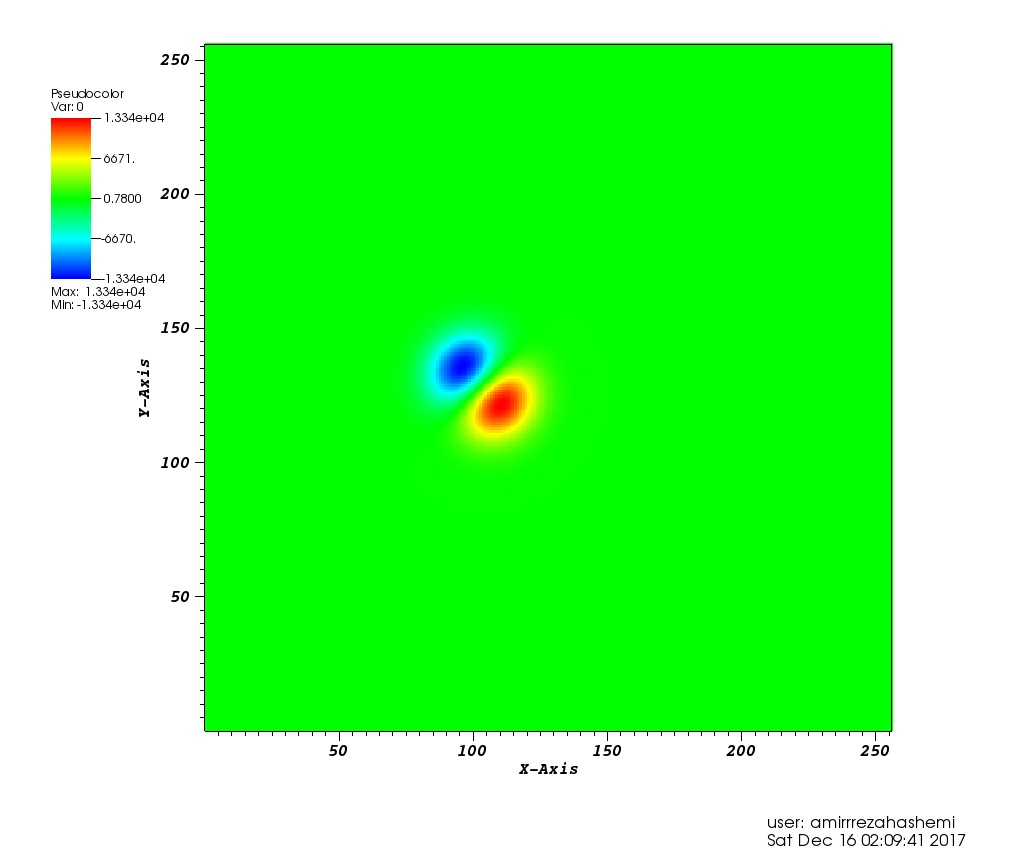
\includegraphics[scale=0.4]{fig1}
     \caption{Vorticity contour at the initial condition.}
   \end{figure}
   
       \begin{figure}
    \centering
     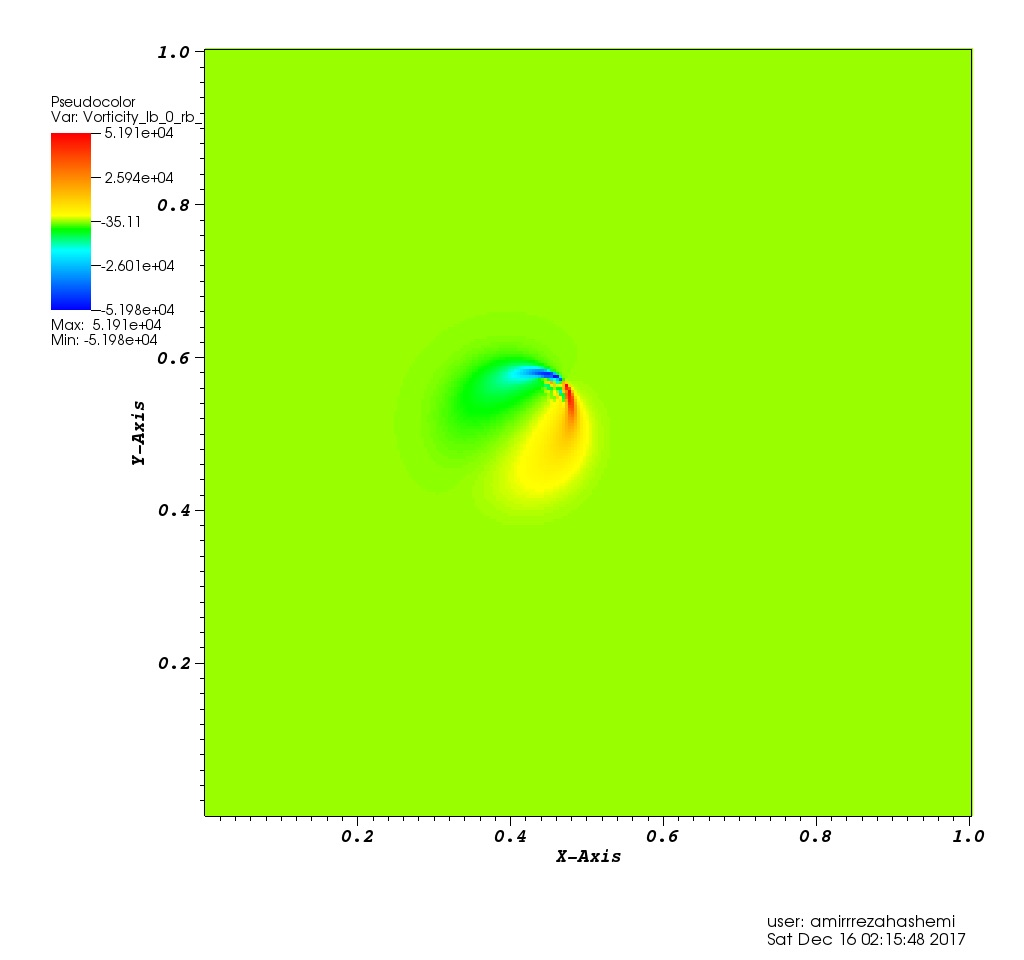
\includegraphics[scale=0.4]{fig2}
     \caption{Vorticity contour before the break down.}
   \end{figure}
\section{Instruction to run}

The executive files for test cases and makefile are located in /Code/exec/. Before running, one would need to build the binaries, which are not included in our submission. The provided GNUmakefile will build the test binaries:
\begin{description}
	\item[AdvectionTest] make AdvectionTest
	\item[BCTest] make BCTest
	\item[BCHLaiTest] make BCHLaiTest
\end{description}

The following commands will run and produce the outcome for each test:
\begin{description}
	\item[AdvectionTest.cpp] ./AdvectionTest2D.exe
	\item[BCTest] ./BCTest.exe
	\item[BCHLaiTest.cpp] ./BCHLaiTest2D.exe
\end{description}

Note that the code is written in a tentative way to be compatible with problems of different dimensions. The variable DIM in the makefile defines the number of dimensions, and it influences the 2D in the filenames above.

The outcome will be in the form of .vtk files as they have been explained earlier, and can be viewed with VisIt. The main resulting figures, in vtk format, are also included in the directory /results.

\bibliographystyle{phjcp}
\bibliography{fourth_milestone}

\end{document}

\end{document}
